\documentclass[12pt]{article}
\usepackage{graphicx}
\usepackage{geometry}
\usepackage{hyperref}
\geometry{a4paper, margin=2.5cm}
\title{Fashion-MNIST 单隐藏层 MLP 分类实验报告}
\author{ }
\date{\today}

\begin{document}
\maketitle

\section{实验目的与任务说明}
本实验基于纯 NumPy 实现单隐藏层多层感知机（MLP），完成 Fashion-MNIST 图像分类任务，涵盖数据加载、模型训练、测试评估、超参数搜索、权重可视化和错例分析等完整流程。

\section{数据集与预处理}
\begin{itemize}
  \item 数据集：Fashion-MNIST，自动下载至 data/ 目录。
  \item 划分：训练集、验证集、测试集，训练集按 9:1 划分出验证集。
  \item 预处理：所有图像归一化到 [0,1]，输入展平成 784 维向量。
\end{itemize}

\section{模型结构与实现}
\begin{itemize}
  \item 结构：单隐藏层 MLP，输入层 784，隐藏层可调（如 256），输出层 10 类。
  \item 激活函数：支持 relu、sigmoid、tanh。
  \item 权重初始化：Xavier 初始化。
  \item 损失函数：交叉熵损失，支持 L2 正则。
  \item 优化器：SGD，支持学习率衰减（exp/cosine）。
  \item 反向传播：手工实现，无深度学习框架依赖。
\end{itemize}
模型结构代码片段（src/hw1/model.py）：
\begin{verbatim}
class OneHiddenLayerMLP:
    def __init__(...):
        ...
\end{verbatim}

\section{训练过程与参数设置}
\begin{itemize}
  \item 训练命令：
\begin{verbatim}
python scripts/train.py --epochs 100 --batch-size 128 --learning-rate 0.05 --lr-decay 0.95 --lr-schedule cosine --min-lr 1e-5 --weight-decay 1e-4 --hidden-dim1 256 --activation relu
\end{verbatim}
  \item 主要参数：epochs=100, batch\_size=128, learning\_rate=0.05, lr\_schedule=cosine, min\_lr=1e-5, weight\_decay=1e-4, hidden\_dim1=256, activation=relu。
  \item 训练过程自动保存最优模型和训练历史。
  \item 训练/验证损失与准确率曲线：
\begin{center}
\includegraphics[width=0.7\textwidth]{artifacts/curves.png}
\end{center}
\end{itemize}

\section{测试集评估}
\begin{itemize}
  \item 测试命令：
\begin{verbatim}
python scripts/test.py --data-dir data --model-path checkpoints/best_model.npz --hidden-dim1 256 --activation relu
\end{verbatim}
  \item 输出：终端打印 Test Accuracy 和 Confusion Matrix，并保存混淆矩阵图片。
  \item 示例：
\begin{center}
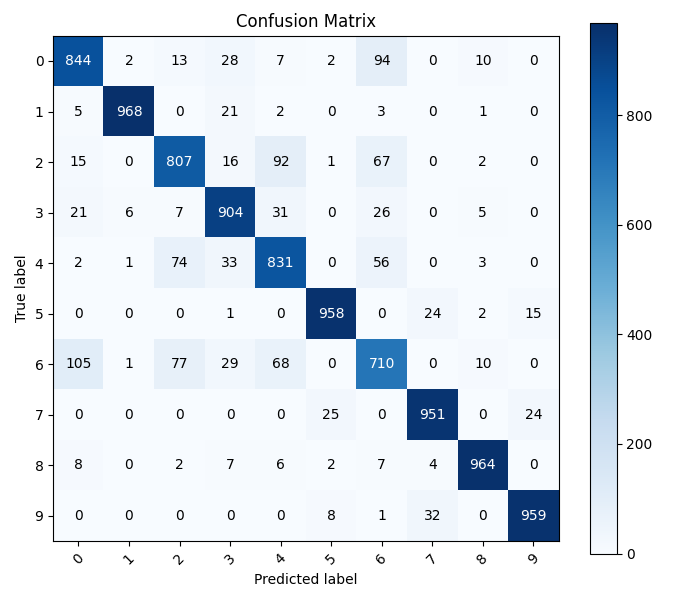
\includegraphics[width=0.5\textwidth]{artifacts/confusion_matrix.png}
\end{center}
\end{itemize}

\section{超参数搜索}
\begin{itemize}
  \item 搜索命令：
\begin{verbatim}
python scripts/search.py --data-dir data --epochs 100 --batch-size 128 --seed 42 --results-path artifacts/search_results.json
\end{verbatim}
  \item 搜索范围：learning\_rate, hidden\_dim1, weight\_decay, activation。
  \item 搜索结果：自动生成每种激活函数的热力图。
\begin{center}
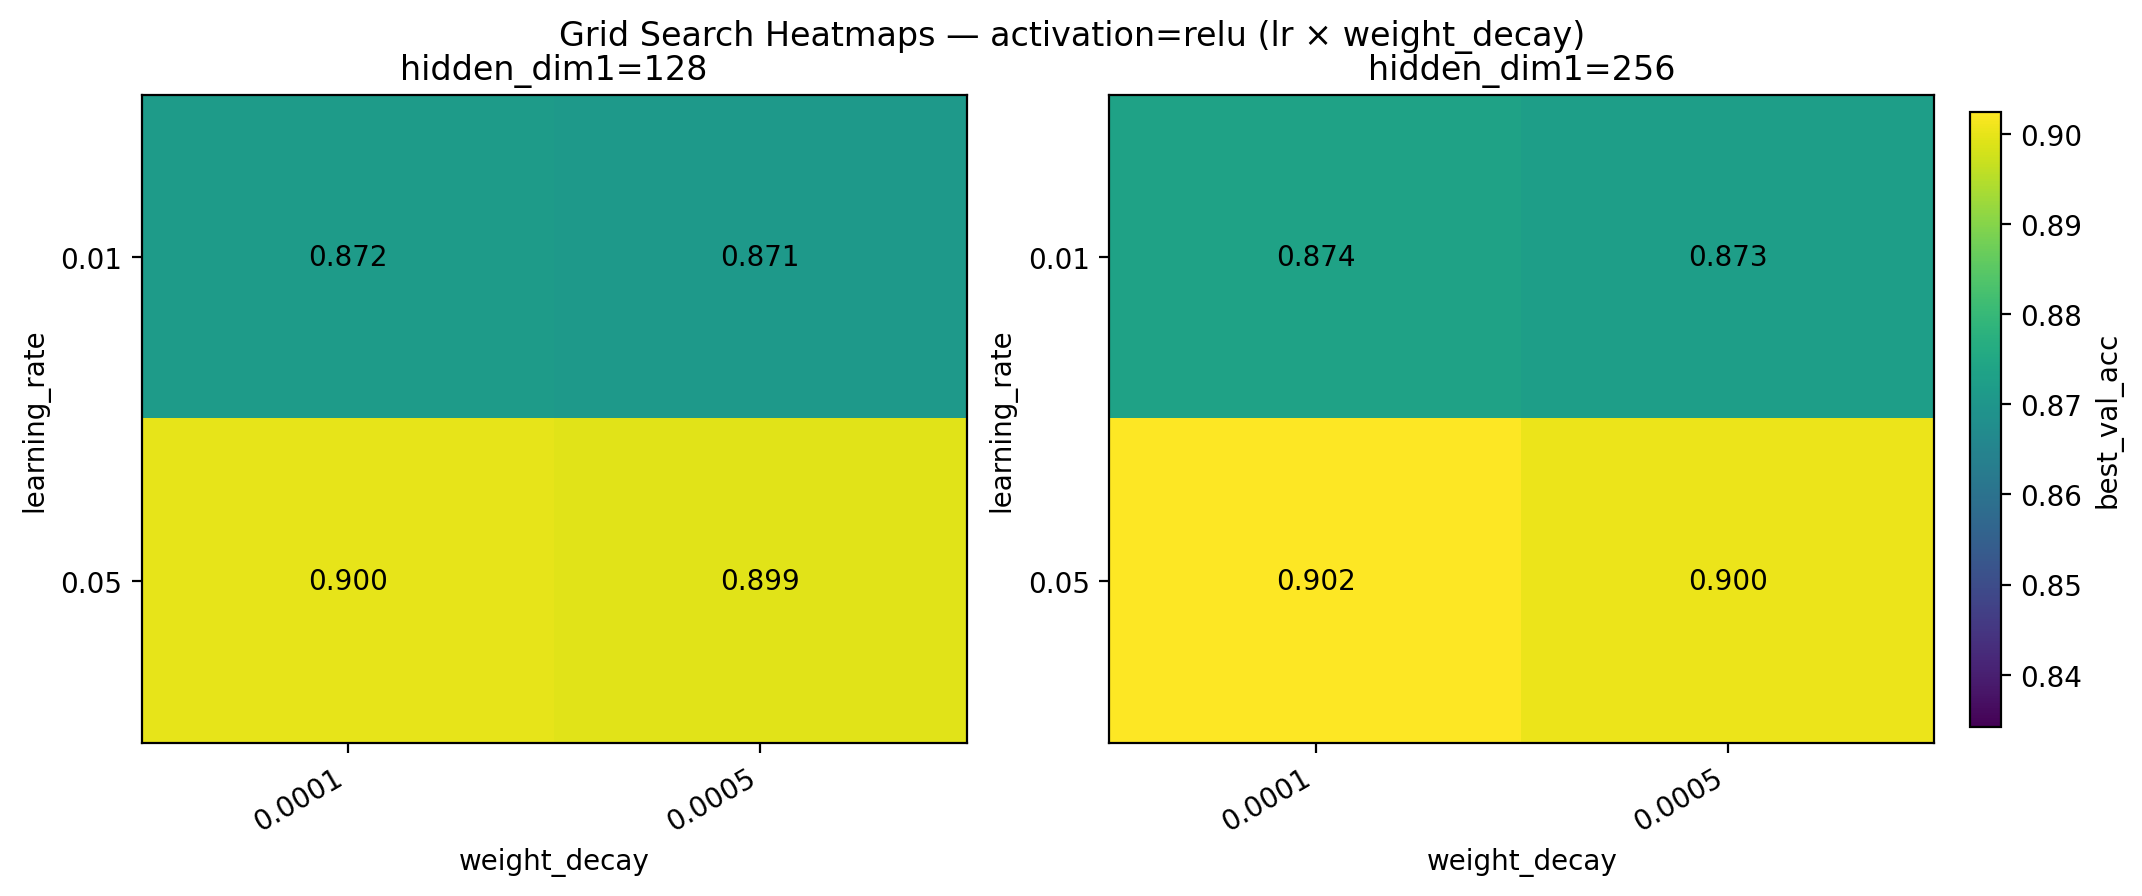
\includegraphics[width=0.5\textwidth]{artifacts/search_heatmap_relu.png}
\end{center}
  \item 可用 plot\_search\_results.py 生成更多对比图：
\begin{verbatim}
python scripts/plot_search_results.py artifacts/search_results.json --all
\end{verbatim}
\end{itemize}

\section{第一层权重可视化}
\begin{itemize}
  \item 可视化命令：
\begin{verbatim}
python scripts/visualize_weights.py --model-path checkpoints/best_model.npz --hidden-dim1 256 --activation relu --num-filters 16
\end{verbatim}
  \item 输出：artifacts/first\_layer\_weights.png
  \item 说明：自动展示对每个类别判别力最强的隐藏单元权重图。
\begin{center}
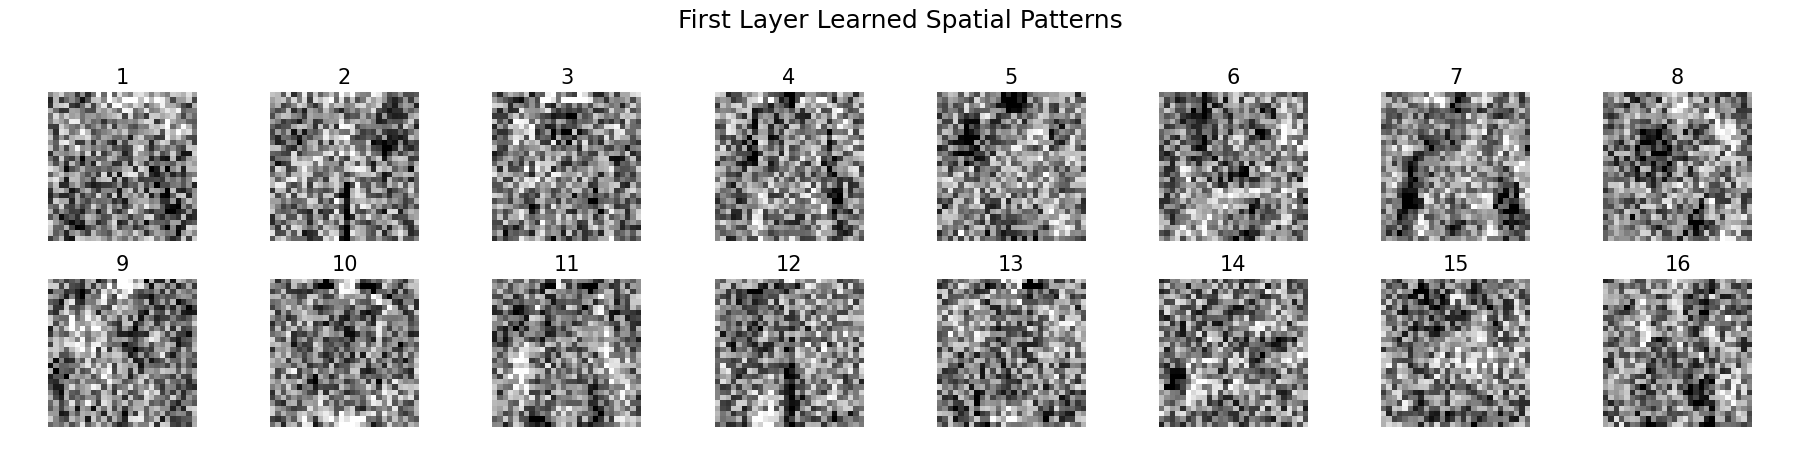
\includegraphics[width=0.7\textwidth]{artifacts/first_layer_weights.png}
\end{center}
\end{itemize}

\section{错例分析}
\begin{itemize}
  \item 错例分析命令：
\begin{verbatim}
python scripts/error_analysis.py --data-dir data --model-path checkpoints/best_model.npz --hidden-dim1 256 --activation relu --num-errors 16 --out-path artifacts/error_cases.png
\end{verbatim}
  \item 输出：artifacts/error\_cases.png
  \item 说明：展示模型预测错误的样本及其真实/预测标签。
\begin{center}
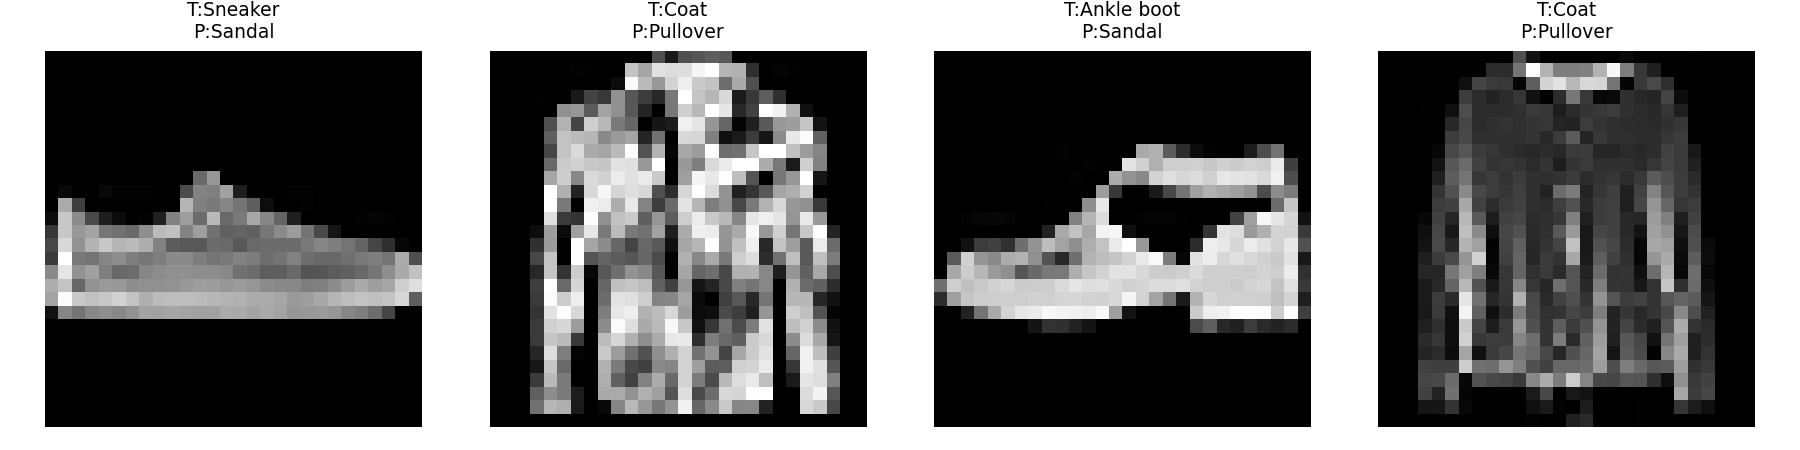
\includegraphics[width=0.7\textwidth]{artifacts/error_cases.png}
\end{center}
\end{itemize}

\section{总结与思考}
\begin{itemize}
  \item 本实验实现了纯 NumPy 下的 MLP 分类器，涵盖完整机器学习实验流程。
  \item 通过超参数搜索和可视化，深入理解了模型结构、参数对性能的影响。
  \item 错例分析帮助发现模型局限和数据集难点。
  \item 后续可尝试更深层网络、不同优化器、数据增强等改进。
\end{itemize}

\section*{附录}
\subsection*{目录结构}
\begin{verbatim}
.
├── scripts/
│   ├── train.py
│   ├── test.py
│   ├── search.py
│   ├── visualize_weights.py
│   └── error_analysis.py
├── src/hw1/
│   ├── data.py
│   ├── model.py
│   ├── train.py
│   └── evaluate.py
└── requirements.txt
\end{verbatim}

\subsection*{主要命令与参数说明}
详见各节命令与参数表。

\end{document}
